
\chapter{Addressing Weakly Coupled Carbon Spins}
\label{chap:addressing_weakly_coupled_carbons}

In order to realize quantum error correction at least three qubits and at least five to correct for a universal error will be needed.
Strongly coupled carbon spins can be controlled as explained in the previous chapter \citep{Robledo2011HighFidelity,Waldherr2014Quantum}.
However the probability of finding enough of these spins to implement QEC is very small.
The probability of finding three or more strongly coupled carbons spins in an NV-center is low and goes down the more carbons are required \citep{Waldherr2014Quantum,Taminiau2014Universal}.
Additionally strongly coupled nuclear spins are prone to decohere when the electronic spin is optically addressed\citep{Pfaff2012Demonstration}.
A problematic feature for QEC which relies on repeatedly measuring errors to be able to correct for them.

By addressing weakly coupled carbon spins the spin register can be enlarged with spins that are not affected as strongly by the readout of the electron spin.
However to address weakly coupled carbon spins the coherence of the electron needs to be extended.
This is done trough dynamical decoupling \citep{Lange2010Universal}.
Van der Sar et al. \citep{Sar2012DecoherenceProtected} have demonstrated how to integrate gates on the nitrogen spin with dynamical decoupling sequences.
To address these weakly coupled carbon spins we use the dynamical decoupling sequence used to extend the coherence \citep{Taminiau2012Detection}.
In the next chapter it is demonstrated how this control is used to perform parity measurements and create entanglement.

In this chapter it will first be explained how the coherence can be extended trough dynamical decoupling so that weakly coupled carbon spins can be addressed.
The dynamical decoupling sequence will then be used to identify spins in the environment.
These spins are characterized so that they can be controlled in the next chapter.


\section{Extending Electron Coherence}

To be able to resolve weakly coupled carbons it is necessary to extend the coherence of the NV-spin.
By using a technique known as a spin-echo the effect of variations in the environment \emph{between} experiments can be eliminated, making variations \emph{during} experiments the main source of decoherence.
By dynamical decoupling the effect of these variations on the coherence can be minimized and the dynamics of the spin-bath exposed.


\subsection{Spin-Echo}

A spin echo experiment (\cref{fig:spin_echo_gijs}) is very similar to a Ramsey experiment.
The difference is an additional $\pi$ pulse that is added in the middle of the experiment exactly between the $\pi/2$ pulses of the Ramsey sequence.
In a spin echo the state is brought into the $xy$-plane where it evolves for a time $\tau/2$ before a $\pi$-pulse, along the y-direction in the rotating frame, is applied.
It evolves for another $\tau/2$ before a final $\pi/2$-pulse rotates it back to $\ket{0}$ and it is read out.

The key component of a spin-echo is the central $\pi$-pulse that cancels out the effect of quasi-static variations in the spin-bath configuration.
The $\pi$-pulse can be seen as turning the reference frame of the NV-spin upside down.
If the spin-bath configuration does not change during the experiment, the detuning of the evolution frequency with respect to the central frequency during the first part will be exactly opposite to the detuning during the second part.
This means that any phase difference picked up during the first half of the evolution is canceled out perfectly during the second half of the evolution.
\begin{figure}[htbp]
    \centering
    \includegraphics{Img/SpinEcho_Gijs.pdf}
    \caption{In a spin echo experiment the qubit is brought into the $xy$-plane of the Bloch-sphere by a $\pi/2$-pulse. Here it freely evolves for a time $\tau/2$ before being flipped by a $\pi$-pulse along the $y$-axis of the rotating frame. It is let to evolve for another $\tau/2$ before a final $\pi/2$ pulse brings is used to read out the $x$-component.
    If the spin-bath configuration does not change during the free evolution time $\tau$ the state vector will end up along the $x$-axis irrespective of the initial spin-bath configuration.
    Figure from \citet{Lange2012Quantum}. }
    \label{fig:spin_echo_gijs}
\end{figure}


Because the spin-bath does not remain static during experiments the cancellation is not perfect, some phase is picked up causing the signal to decohere.
Similar to a Ramsey experiment this can be measured by applying a detuning to the rotating frame and measuring the decay of the oscillation.
$T_2$ is defined as the $1/e$ value of the decay of a spin echo experiment and measures decoherence due to variations in the spin-bath during an experiment.
$T_2$ was measured to be $1.10 \pm 0.01 \mathrm{ms}$.
% Data from exp:  20140405/123712

\subsection{Dynamical Decoupling}
A natural way to extend the phase cancellation properties of the spin-echo experiment to shorter timescales is by applying more $\pi$-pulses.
This procedure is known as dynamical-decoupling.
Similar to how the spin-echo cancels out phase picked up due to any variations that are quasi-static on the time-scale of the experiment, dynamical-decoupling cancels out phase due to variations on the time-scale of the $\pi$-pulses.
Dynamical-decoupling can dramatically improve coherence times\citep{Lange2010Universal}.

On our sample a coherent signal\footnote{$F\ket{0} > 0.68$} is measured after more than $40 \mu$s for 256 pulses.
Work on ensembles indicates that that this can be improved even further by applying more pulses: a coherence time of $T_{DD} \approx 0.6 \mathrm{s}$ was reported at 77K \citep{Gill2013SolidState}.

\subsection{Dynamical decoupling spectroscopy}

When discussing the Ramsey and the spin-echo experiment we have treated the NV-center as being affected by the spin-bath but not interacting with it.
In reality the NV-spin does interact with nuclear spins.
It is possible to probe these interactions using a dynamical decoupling spectroscopy.
During a dynamical decoupling spectroscopy a fingerprint of the spin environment is constructed.

In a dynamical decoupling spectroscopy experiment the electron is prepared in the $|X\rangle =\tfrac{1}{\sqrt{2}}\left( |0\rangle +|1\rangle \right) $ state.
It is subjected to a pulse sequence consisting of $N/2$ blocks of the form {$\tau - \pi -2\tau-\pi-\tau$}, where $\tau$ is a wait time and $\pi$ a $\pi$-pulse.
The experiment is concluded by measuring $\langle X\rangle $.
The fingerprint is the result of many repetitions for a range of inter-pulse delays $2\tau$.

Part of a dynamical decoupling spectroscopy can be seen in \cref{fig:FP}.
When the central spin interacts conditionally with a spin in the environment coherence is lost when the central spin is measured.
In a fingerprint such an interaction is visible as a lowered contrast.

% The spectroscopy was performed for N = 8, 16, 32 and 64 pulses. For N = 8, 16 and 32 pulses this was done between $\tau = 2 \mu \mathrm{s}$  and $72 \mu \mathrm{s}$ and for N = 64 this was done up to $\tau = 52 \mu \mathrm{s}$. A reference to the full spectroscopy can be found in \cref{chap:Fingerprint_data_appendix}.

\begin{figure}[htbp]

    \begin{subfigure}[t]{\textwidth}\centering
        \caption{}
        \begin{tikzpicture}
            \node[anchor=south west,inner sep=0] at (0,0) {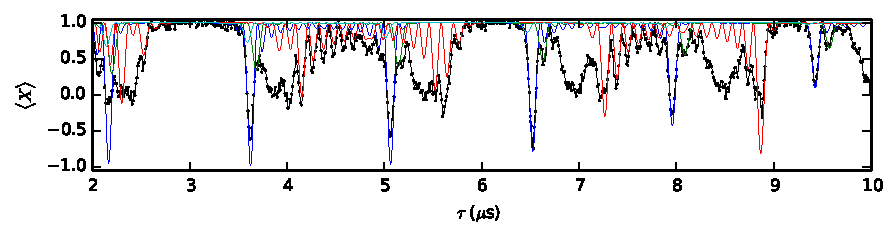
\includegraphics{Img/fingerprint16.pdf}};
            \node[font=\small, text = blue] at (4.05,1.7)  {1};
            \node[font=\small, text = green] at (9.3,2.9) {2};
            \node[font=\small, text = red] at (5.3,2.5) {3};
            \node[font=\small, text = cyan] at (4.0,3.35) {4};
            \node[font=\small, text = black] at (14.0,4.0) {$N=16$};
            % \draw[help lines,xstep=1,ystep=1] (0,0) grid (10,3);
            % \foreach \x in {1,2,...,10} { \node [anchor=north] at (\x,0) {\x}; }
            % \foreach \y in {1,2,...,3} { \node [anchor=east] at (0,\y) {\y}; }
        \end{tikzpicture}
        \label{fig:FP16}
    \end{subfigure}

    \begin{subfigure}[t]{\textwidth}\centering

    \caption{}
    \begin{tikzpicture}
        \node[anchor=south west,inner sep=0] at (0,0) {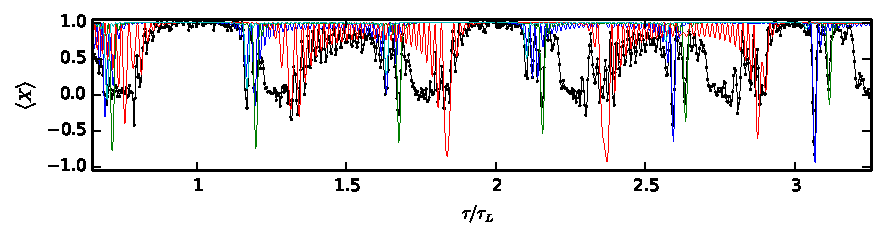
\includegraphics{Img/fingerprint32.pdf}};
        \node[font=\small, text = blue] at (11.2,1.9) {1};
        \node[font=\small, text = blue] at (4.0,2.8)  {1};
        \node[font=\small, text = green] at (6.6,1.8) {2};
        \node[font=\small, text = red] at (7.4,1.8) {3};
        \node[font=\small, text = cyan] at (4.05,2.5) {4};
        \node[font=\small, text = black] at (14.0,4.0) {$N=32$};
        % \draw[help lines,xstep=1,ystep=1] (0,0) grid (10,3);
        % \foreach \x in {1,2,...,10} { \node [anchor=north] at (\x,0) {\x}; }
        % \foreach \y in {1,2,...,3} { \node [anchor=east] at (0,\y) {\y}; }
    \end{tikzpicture}
    \label{fig:FP32}
    \end{subfigure}
    \caption{Part of a fingerprint resulting from a dynamical-decoupling-spectroscopy experiment performed at $B_z = 304\mathrm{G}$, $\tau_L =3.07 \mu \mathrm{s} $. Contrast is lowered when the decoupling sequence performs a conditional operation on a spin in the environment.  A reference to the full spectroscopy can be found in \cref{chap:Fingerprint_data_appendix}.  Black lines correspond to data. Colored lines represent computed responses of carbon spins. Responses were calculated using \cref{eq:contrast_single_carbon_spin} with hyperfine parameters from \cref{tbl:HF_par}. }
    \label{fig:FP}
\end{figure}



% Although dynamical-decoupling improves the coherence of the central spin by decoupling from the environment, the central spin is also decoupled from other spins preventing direct two-qubit gates. It was demonstrated by \citet{Sar2012DecoherenceProtected} how to incorporate dynamical decoupling in a universal gate design by implementing Grover's algorithm.
% Using this technique \citet{Taminiau2012Detection} used the extended coherence to detect and control weakly-coupled carbon spins, before implementing three-qubit quantum-error-correction (QEC) \citep{Taminiau2014Universal}.

% As these experiments where performed with NV-centers at Room temperature they lack the option to do single-shot readout required to act on a measurement outcome\footnote{@Tim, I think this can be worded more concisely. Do you have any ideas?}. An essential feature for the parity measurements that form the basis of measurement-based QEC and surface codes.

% As we cannot perform an ESR experiment while decoupling a different technique must be used to resolve and address additional spins.
% In order to resolve additional spins we perform a dynamical decoupling spectroscopy, resulting in a fingerprint of the nuclear-spin environment\citep{Taminiau2012Detection}.

\section{Identifying weakly-coupled carbon-pins}
To be able to control weakly coupled spins the interaction between these spins and the NV-center must be understood.
This section will discuss the effect of dynamical decoupling on the interaction between the NV-center and weakly coupled nuclear spins.
This knowledge is used to explain the features in the fingerprint of \cref{fig:FP} and identify several nuclear spins.

\subsection{The effect of dynamical decoupling on weakly coupled nuclear spins}

During dynamical decoupling the electronic state alternates between the $m_s = 0$ and $m_s =+1$ state, this causes the nuclear spin to alternately rotate around two distinct quantization axes (\cref{fig:quantax}).
When the electron is in the $m_s=0$ state each nuclear spin precesses about $\bm{\omega_L}$ with the Larmor frequency.
When the electron is in the $m_s=+1$ state there is a hyperfine interaction between the nucleus and the NV-center (\cref{eq:nuclear_hamiltonian_1}) and the spin precesses around $\bm{\tilde{\omega}}=\bm{\omega_L} +\bm{A}$, where $\bm{A} = A_\parallel \bm{\hat{z}} + A_\perp \bm{\hat{x}}$ \citep{Taminiau2012Detection}.


\begin{figure}[htbp]
\centering

        \begin{tikzpicture}
            \node[anchor=south west,inner sep=0] at (0,0) {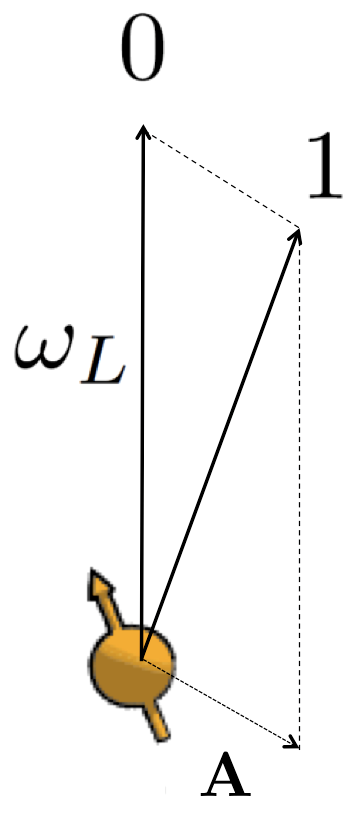
\includegraphics[keepaspectratio,width=0.15\textwidth]{./img/QuantizationAxis.png}};
            \node[font=\huge, text = black] at (1.6,2.0)  {${\tilde{\omega}}$};
        \end{tikzpicture}
\caption{Flipping the electron spin from the  $m_s=0$ to the $m_s= +1$ state changes the quantization axis of nuclear spins. For  $m_s=0$ all nuclear spins precess about $\bm{\omega_L}$. For  $m_s=+1$ each spin precesses about a distinct axis $\bm{\tilde{\omega}}=\bm{\omega_L} +\bm{A}$.}
\label{fig:quantax}
\end{figure}

The result of a decoupling sequence is a net rotation around an axis $\bm{\hat{\mathrm{n_i}}}$ by an angle $\theta$.
Where $\bm{\hat{\mathrm{n_i}}}$ depends on the initial state of the electron and $\theta$ is proportional to the number of pulses $N$ \citep{Taminiau2012Detection}.
$\bm{\hat{\mathrm{n_i}}} =\bm{\hat{\mathrm{n_0}}}$ when the electron starts in $m_s = 0$ and $\bm{\hat{\mathrm{n_i}}} =\bm{\hat{\mathrm{n_1}}}$ when the electron starts in $m_s = +1$.

\begin{figure}[htbp]
    \begin{subfigure}[t]{0.49\textwidth}\centering
        \centering
        \caption{}
        \includegraphics{Img/unCond_rot_taminiau.pdf}
        \label{fig:uncond_rot}
    \end{subfigure}
    \begin{subfigure}[t]{0.49\textwidth}\centering
        \centering
        \caption{}
        \includegraphics{Img/Cond_rot_taminiau.pdf}
        \label{fig:cond_rot}
    \end{subfigure}
    \caption{\Cref{fig:uncond_rot} When the net rotation axes $\bm{\hat{\mathrm{n_0}}}$ and $\bm{\hat{\mathrm{n_1}}}$ point in the same direction the carbon experiences an unconditional rotation and cannot be controlled. \Cref{fig:cond_rot} When the net rotation axes $\bm{\hat{\mathrm{n_0}}}$ and $\bm{\hat{\mathrm{n_1}}}$ are anti-parallel the carbon experiences a conditional rotation, either around $+x$ or $-x$, and can be controlled. Figure from \citep{Taminiau2012Detection}.}
    \label{fig:conditional_and_unconditional_rotation}
\end{figure}

When the net rotation axes point in a different direction a conditional operation is executed during dynamical decoupling (\cref{fig:conditional_and_unconditional_rotation}).
In a dynamical decoupling spectroscopy contrast is lost when a conditional operation is executed.
To understand when this occurs it is useful to consider three different cases.
A weakly coupled carbon spin in: the \emph{trivial} regime where $A_\perp=0$, the \emph{basic} regime where $A_\perp \ll \omega_L$ and the \emph{complex} regime where $A_\perp \sim \omega_L$.
For a complete mathematical description of the response of nuclear spins to a dynamical decoupling spectroscopy the reader is referred to \cref{sec:mathematical_description_dd_spectro}.

\subsubsection{The trivial regime ($A_\perp=0$)}
Because there is no orthogonal component of the hyperfine the spin will precess around the $z$-axis independent of the initial electronic spin-state.
Therefore no conditional operation is possible and it is not possible to resolve such a spin in a dynamical decoupling spectroscopy.

\subsubsection{The basic regime ($A_\perp \ll \omega_L$)}
In the basic regime the net rotation axes are practically parallel and point in the $z$-direction for almost every $\tau$ except for a specific resonant condition for which the axes are anti-parallel.
This resonant condition is given by \cref{eq:res_dip_loc}, where $k$ is an integer, and has a Lorentzian shape in a dynamical decoupling spectroscopy.
The FWHM of the resonance is given by \cref{eq:res_dip_width}.

 \begin{equation}
\tau = \frac{(2k+1)\pi}{2 \omega_L + A_\parallel}
\label{eq:res_dip_loc}
\end{equation}
 \begin{equation}
\mathrm{FWHM_{DD}} = \frac{A_\perp}{2 \omega_L^2}
\label{eq:res_dip_width}
\end{equation}

\subsubsection{The complex regime ($A_\perp \sim \omega_L$)}

In the case where $\bm{\omega_L}$ and $\bm{A_\perp}$ are of comparable magnitude the net rotation axes $\bm{\hat{\mathrm{n_i}}}$ are strongly dependent on the initial electron-state for almost any $\tau$.
When a carbon is in the complex regime it is no longer possible to describe it as a narrow resonance in the dynamical decoupling spectroscopy.
The response is visible as a wide resonance with an oscillation on top of it.

\paragraph{}
Because the electron is not interacting with a single carbon but with a bath of carbon atoms the contrast $M$ is given by the product of all individual values $M_j$ for each individual spin $j$ (\cref{eq:prod_multiple_spins}).
When the responses of multiple carbons overlap contrast is quickly lost.
\begin{equation}
\label{eq:prod_multiple_spins}
    M = \prod_{j}{M_j}
\end{equation}

In order to distinguish an individual carbon-spin its response must not overlap with that of other carbon spins.
By sweeping the number of $\pi$-pules the response of an individual carbon can be distinguished from the response of multiple spins.
Only when an individual spin is being addressed is it possible to sweep the contrast of the dynamical decoupling spectroscopy to -1 by increasing the number of pulses.

\subsection{Identifying Individual Carbon-spins}
Going back to \cref{fig:FP} it is now possible to explain its features.

A broad feature with low coherence is clearly visible around $\tau/(4\tau_L) = m$ for odd $m$.
This feature is known as the spin-bath collapse and is caused by the response of multiple spins overlapping.

At the edges of the spin bath several sharp dips are visible. These most likely correspond to individual spins.
A first estimate of the hyperfine coupling to these spins can be made based on their location and width using \cref{eq:res_dip_loc,eq:res_dip_width}.

Between the spin-bath collapses there alternately appears an oscillation.
This oscillation is most likely caused by a spin in the complex regime.
It's position can be used to get a rough estimate for its hyperfine coupling.

By computing the responses for these estimated hyperfine parameters using \cref{eq:contrast_single_carbon_spin} a more accurate estimation can be made.
The parameters are varied until the computed response agrees with the data as well as possible.
Using this method 13 distinct carbon spins where identified.

The parameters of the 4 strongest coupled carbons are listed in \cref{tbl:HF_par} and their computed responses are visible as colored lines in \cref{fig:FP}.
All estimated hyperfine parameters and a link to the full fingerprint measurements can be found in \cref{chap:Fingerprint_data_appendix}.

\begin{table}[htbp]
\centering
    \begin{tabular}{cllll}
    Carbon & \quad \quad  $A_{\parallel} $ & \quad \quad $A_{\perp}$ \\ \hline
    1         & $2 \pi \cdot${ }30.0 kHz             & $2 \pi \cdot${ }80.0 kHz                \\
    2         & $2 \pi \cdot${ }27.0 kHz             & $2 \pi \cdot${ }28.5 kHz              \\
    3         & $2 \pi \cdot$-51.0 kHz          & $2 \pi \cdot$105.0 kHz              \\
    4         & $2 \pi \cdot${ }45.1 kHz           & $2 \pi \cdot${ }20.0 kHz                \\
    \end{tabular}
    \caption{Estimated hyperfine parameters for spins 1 to 4 in \cref{fig:FP}.}
    \label{tbl:HF_par}
\end{table}


\section{Characterizing weakly-coupled carbon spins}
Using the knowledge of the interaction between the NV-center and individual nuclear spins it is possible to implement basic gates and characterize the spins.
This section will first explain how basic gates can be implemented on weakly coupled carbon spins.
These gates are then used to measure the precession frequency and $T_2*$ for individual carbon spins.

\subsection{Basic operations}
In order to implement basic gates on a nuclear spin we make use of the conditional rotation that occurs on the resonance given by \cref{eq:res_dip_loc}.
At the resonant condition the nuclear spin rotates about one of two anti-parallel axes depending on the electronic-spin state.
The angle of the rotation is proportional to the number of pulses on the electron ($N$).
By sweeping the number of pulses to perform a $\pi/2$ rotation a maximally entangling gate is performed.
We define the axis of rotation of this operation as the $x$-axis and call the operation the $\pm \mathrm{x}$-gate.

By bringing the electron in a superposition, sweeping the number of pulses on the electron and measuring the contrast an oscillation can be measured.
This oscillation can be used to calibrate the $\pm \mathrm{x}$-gate.
For twice the number of pulses ($N_{\pm\mathrm{x}}$) required to implement the $\pm \mathrm{x}$-gate the contrast is -1 for an ideal $\pm \mathrm{x}$-gate.
The fidelity with which the oscillation can be swept to -1 is equal to the squared fidelity with which the $\pm \mathrm{x}$-gate can be implemented.

The $\pm\mathrm{x}$-gate forms the basis of our control over weakly coupled spins.
\Cref{fig:gate_circuit_pm-x} shows how the $\pm \mathrm{x}$-gate is depicted in a circuit-diagram.
A non entangling rotation can be implemented by placing the electron in an eigenstate before performing the $\pm\mathrm{x}$-operation.
By letting the phase of the carbon evolve we are able to apply operations on the carbon-spin with arbitrary phase.


\begin{figure}[htbp]
    \centering
        \mbox{
        \Qcircuit @C=1em @R=.7em {
         \lstick{\ket{\Psi}_e} &\ctrl{1}  &\qw\\
          \lstick{\ket{\Psi}_\mathrm{C}} &\gate{\pm \mathrm{x} }  &\qw}}
    \caption{The $\pm\mathrm{x}$-gate performs an x-rotation on the carbon ($\ket{\Psi}_\mathrm{C}$) when the electron is in the $\ket{0}_e$-state. It performs a $-\mathrm{x}$-rotation when the electron is in the $\ket{1}_e$-state.}
    \label{fig:gate_circuit_pm-x}
\end{figure}

The $\pm\mathrm{x}$-gate has been calibrated for several spins.
The parameters used to implement $\pm\mathrm{x}$-gates are listed in \cref{tbl:gate_parameters}.
Of these carbon-1 and carbon-4 were selected for the experiments.

\begin{table}[htbp]
    \centering
    \caption{Parameters used to implement $\pm\mathrm{x}$-gates.}
    \begin{tabular}{cccc}
    Carbon &  $ N $ &  $\tau$ & total gate time\\ \hline
    1 &  18 & { }9.420 $\mu$s & 339 $\mu$s \\
    2 & 26 & { }6.620 $\mu$s & 344 $\mu$s \\
    3 & 14 & 18.564 $\mu$s & 520 $\mu$s \\
    4 &  40 & { }6.456 $\mu$s & 516 $\mu$s
    \end{tabular}
    \label{tbl:gate_parameters}
\end{table}



\subsection{Carbon Ramsey experiment }
By performing a Ramsey experiment the precession and dephasing-time $T_2^*$ can be determined.
The precession frequencies are required to calculated the phase required to implement operations with the correct phase.
By measuring the precession frequency it is also possible to test our estimation for the hyperfine parameters.

In an ordinary Ramsey experiment a qubit is brought to the equator of the Bloch-sphere where it precesses for a time $\tau $ before it is read out along the x-direction.
A carbon-Ramsey experiment is similar.
\begin{figure}[htbp]
        \centering
        \mbox{
        \Qcircuit @C=1em @R=.7em {
        \lstick{\ket{0}}          & \gate{\mathrm{y}}  & \ctrl{1}    & \dashedGate{\mathrm{x}}  & \multigate{1}{T}  & \dashedGate{\mathrm{-x}}      &\ctrl{1}          & \gate{\mathrm{-y}}  &  \meter \\
        \lstick{\rho_\mathrm{m}}         & \qw              &  \gate{\pm \mathrm{x}}    &  \qw& \ghost{T}        & \qw & \gate{\pm \mathrm{x}}      & \qw       &\qw&}}
    \caption{Gate circuit depicting an uninitialized carbon Ramsey. $T$ is the free evolution time. $\mathrm{x}$ and $\mathrm{y}$ are $\pi/2$ pulses along the $x$ and $y$ axis respectively. The dotted gates are not present when the electron is protected against decoherence by dynamical decoupling during the free evolution time $T$.}
    \label{fig:gate_circuit_nuclear_ramsey}
\end{figure}

The gate circuit of the uninitialized carbon-Ramsey experiment is depicted in \cref{fig:gate_circuit_nuclear_ramsey}.
The first pulse brings the electronic spin in the $\ket{X}$-state.
Because the carbon starts out in a mixed state the two-qubit system can be described by the tensor product of two density matrices:
\begin{equation}
    \rho_X \otimes \rho_m = \rho_X \otimes \rho_{X} +\rho_X \otimes \rho_{-X}
\end{equation}
By applying the $\pm{\mathrm{x}}$-gate  the electronic-spin picks up a phase depending on the nuclear spin-state:
\begin{equation}
     \rho_Y \otimes \rho_{X} +\rho_{-Y} \otimes \rho_{-X}
    \label{eq:density_after_Ren}
\end{equation}
In this state it is either left to freely evolve for a time $T$ while the electronic spin is protected against decoherence trough dynamical decoupling, or a $\pi/2$-pulse is applied to bring the electron back to the poles of the Bloch-sphere.
If the extra $\pi/2$-pulse is applied the system is in the following state before the free evolution.
\begin{equation}
     \rho_0 \otimes \rho_{X} +\rho_{1} \otimes \rho_{-X}
\end{equation}
Because the electronic spin is in a different state for $\rho_{X}$ and $\rho_{-X}$ they evolve with different frequencies.
After the free evolution another $\pi/2$-pulse is applied to bring the electronic spin back into the $xy$-plane.

The final part of the circuit reads out the nuclear spin along the $x$-direction for $\ket{Y}_e$ and along the $-x$-direction for $\ket{-Y}_e$.
The phase picked up during free evolution shows up as an oscillation between $\ket{0}_e$ and $\ket{1}_e$ in the readout.

\subsubsection{Determining the precession frequency}
Because the uninitialized carbon-Ramsey evolves with two frequencies we expect the measured oscillation to be the sum of two cosines as described by \cref{eq:carbon_ramsey_expected}:
\begin{equation}
    c_1 - c_2 \cos(\omega_L \tau ) -c_3  \cos (\tilde{\omega} \tau )
    \label{eq:carbon_ramsey_expected}
\end{equation}
Where $ \tilde\omega =   \sqrt{(\omega_L+A_\parallel) ^2 + A_\perp^2} $ and $c_1$, $c_2$ and $c_3$ are constants.


\begin{figure}[htbp]
    \begin{subfigure}[t]{0.49\textwidth}\centering
        \caption{}
        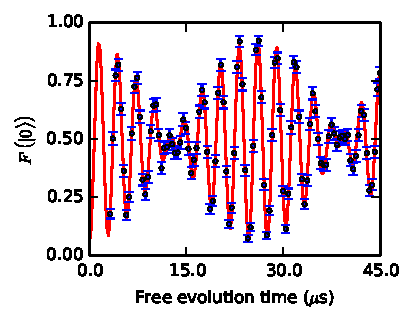
\includegraphics{Img/CarbonRamsey_C1.pdf}
        \label{fig:CR_C1}
    \end{subfigure}
    \begin{subfigure}[t]{0.49\textwidth}\centering
        \caption{}
        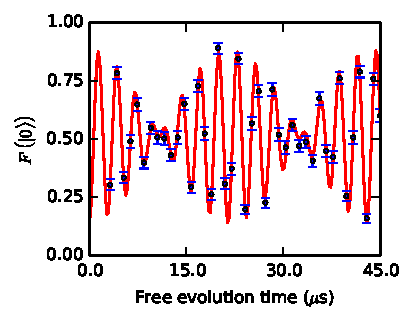
\includegraphics{Img/CarbonRamsey_C4.pdf}
        \label{fig:CR_C4}
    \end{subfigure}
    \caption{The uninitialized carbon-Ramsey experiment shows an oscillation due to the phase picked up during free evolution.
    \subref{fig:CR_C1} shows data for carbon-1 and \subref{fig:CR_C4} for carbon-4.
    The measured frequencies were, for carbon-1: $\omega_{L,C1} = 2\pi\cdot 325.81 \pm 0.25$ and  $\tilde \omega_{\mathrm{C1}}= 2\pi\cdot 364.41 \pm 0.23$, and for carbon-4: $\omega_{L,C4} =  2\pi\cdot 325.94 \pm 0.40$ and $\tilde \omega_{\mathrm{C4}} = 2\pi\cdot 371.52 \pm 0.39 $.}
    \label{fig:Uninitialized_carbon_ramsey}
\end{figure}

\Cref{fig:Uninitialized_carbon_ramsey} shows the results for an uninitialized carbon-Ramsey experiment.
The data was fitted to a sum of two cosines in order to determine the frequencies.

The Larmor frequencies measured are $\omega_{L,C1} = 2\pi\cdot 325.81 \pm 0.25\, \mathrm{kHz}$  for carbon-1 and  $\omega_{L,C4} =  2\pi\cdot 325.94 \pm 0.40\, \mathrm{kHz}$for carbon-4.
Both the measured Larmor frequencies agree with the magnetic field of $304\, \mathrm{G}$ within two standard deviations.

Based on the estimated hyperfine parameters we expect $\tilde\omega_{\mathrm{C1}} \approx 2\pi\cdot 364.7\, \mathrm{kHz}$for carbon-1 and $\tilde \omega_{\mathrm{C4}} \approx 2\pi\cdot 371.4\, \mathrm{kHz}$ for carbon-4.
For carbon-1 $\tilde \omega_{\mathrm{C1}}= 2\pi\cdot 364.41 \pm 0.23\, \mathrm{kHz}$ was measured
and for carbon-4 $\tilde \omega_{\mathrm{C4}} = 2\pi\cdot 371.52 \pm 0.39 \, \mathrm{kHz}$ was measured.
Both these values are in good agreement with experiment, an indication that our hyperfine estimation is accurate.


\subsubsection{Measuring $T_{2,\mathrm{C}}^* $}
% Lange carbon ramseys van Hans sil01 140506 #53 en 56 +T2* analyse.
% hoeveel pulses voor de lange tau? belangrijk voor T2*
To determine $T_{2,\mathrm{C}}^* $ for normal operation an uninitialized carbon-Ramsey was performed where the electron was dynamically decoupled during the free evolution time.
Dynamical decoupling was performed at $\tau = 8\cdot \tau_L$ by varying the number of pulses $N$. $\tau_L$ is the Larmor period $1/\omega_L$ of the carbon.
Because the electron is constantly flipped the carbon will precess with an average frequency of $\omega_{\mathrm{DD}} = (\omega_L +\tilde{\omega} )/2$.
By undersampling with a frequency slightly detuned from the precession frequency ($\omega_{\mathrm{DD}}$) a decaying cosine can be observed where the 1/e time of the envelope is equal to $T_2^*$.
Because this decaying cosine can be measured for a relatively long time ($\sim \mathrm{ms}$) this method can also be used to accurately determine the precession frequency.

\begin{figure}[htbp]
    \begin{subfigure}[t]{0.49\textwidth}\centering
        \caption{}
        \includegraphics{Img/Carbon1_T2star.pdf}
        \label{fig:T2star_carbon1}
    \end{subfigure}
    \begin{subfigure}[t]{0.49\textwidth}\centering
        \caption{}
        \includegraphics{Img/Carbon4_T2star.pdf}
        \label{fig:T2star_carbon4}
    \end{subfigure}
    \caption{Carbon-Ramsey experiment to determine $T_2^*$ for nuclei while decoupling the electron.
    Dynamical decoupling during evolution is implemented at $8\cdot \tau_L$ of the carbon spin. Free evolution time is varied by varying the number of pulses.
    The decays are fitted with a generalized normal distribution to determine $T_2^*$ and the exponent $n$.
    \subref{fig:T2star_carbon1} Ramsey decay for carbon-1, $T_{2,\mathrm{C1}}^* =9.85 \pm   0.39 \, \mathrm{ms}$ and $n= 1.83 \pm 0.19$.
    \subref{fig:T2star_carbon4} Ramsey decay for carbon-4,  $T_{2,\mathrm{C4}}^* =6.68 \pm   0.22 \, \mathrm{ms}$ and $n= 2.31 \pm 0.31$. } %would like to add that not limited by electron coherence due to DD.
    \label{fig:T2star_carbon}
\end{figure}

\Cref{fig:T2star_carbon} shows the decay for both carbons.
The decay follows a Gaussian profile within uncertainty for both spins.
The coherence times measured were $T_{2,\mathrm{C1}}^* =9.85 \pm   0.39 \, \mathrm{ms}$ for carbon-1 and $T_{2,\mathrm{C4}}^* =6.68 \pm   0.22 \, \mathrm{ms}$ for carbon-4.
It should be noted that these $T_2^*$ values are not limited by the electron coherence which was measured to be larger than $40 \,\mathrm{ms}$ for $N=256$ pulses.



